\documentclass[english,11pt,openany]{article}
\usepackage{graphicx}
\usepackage{float}
\usepackage{subcaption}
\usepackage{ucs}
\usepackage{bbm}
\usepackage[utf8]{inputenc}
\usepackage[executivepaper,margin=1in]{geometry}
%\usepackage[charter]{mathdesign}
\usepackage{babel}
% \usepackage{subfigure}
\usepackage{fancyhdr}
\usepackage{listings}
\usepackage{lmodern}
\usepackage{amsmath}
\usepackage{empheq}
\usepackage{amsthm}
\usepackage{algorithm}
\usepackage{algpseudocode}
\usepackage{pifont}
\theoremstyle{definition}
\newtheorem{defn}{Definition}[section]
\newcommand{\E}{\mathbb{E}}
\newcommand{\R}{\mathbb{R}}
\newcommand{\bigO}{\mathcal{O}}
\usepackage[toc,page]{appendix}
\renewcommand{\baselinestretch}{1.3}

\usepackage{booktabs}
\usepackage[svgnames,table]{xcolor}
\usepackage[tableposition=above]{caption}
\usepackage{pifont}

\usepackage{afterpage}

\newcommand\blankpage{%
	\null
	\thispagestyle{empty}%
	\addtocounter{page}{-1}%
	\newpage}

\theoremstyle{plain}
\newtheorem{Th}{Theorem}[section]
\newtheorem{Lemma}[Th]{Lemma}
\newtheorem{Cor}[Th]{Corollary}
\newtheorem{Prop}[Th]{Proposition}

\theoremstyle{definition}
\newtheorem{Def}[Th]{Definition}
\newtheorem{Conj}[Th]{Conjecture}
\newtheorem{Rem}[Th]{Remark}
\newtheorem{?}[Th]{Problem}
\newtheorem{Ex}[Th]{Example}

\newtheorem{theorem}{Theorem}
\usepackage{amssymb}
\usepackage[colorlinks=true]{hyperref} 
\hypersetup{urlcolor=blue,linkcolor=black,citecolor=black,colorlinks=true}
%\usepackage[usenames,dvipsnames,svgnames,table]{xcolor}
\definecolor{light-gray}{gray}{0.70}

\begin{document}
	\begin{titlepage}
		
		\title{
			\hspace{0.75cm}Backward Stochastic Differential Equation 
			\newline
			\hspace{0.35cm}\textbf{High Dimensional BSDE}
		}
		
		\author{Majdi Rabia}
		\date{
			\hspace{2.5cm} 
			\newline
		}
		
		\maketitle
		
		
		
		%\hspace{1cm} \includegraphics[width=10cm]{}
		
	\end{titlepage}
	
	
	\blankpage
	
	\section*{Declaration}
	\addcontentsline{toc}{section}{Declaration}
	
	This MSc thesis is an account of research undertaken between December 2015 and 
	April 2017 at The Department of Statistics and Applied Probability, 
	The National University of Singapore, Singapore.
	
	Except where acknowledged in the customary manner, the material 
	presented in this thesis is, to the best of my knowledge, original and 
	has not been submitted in whole or part for a degree in any 
	university.
	
	\vspace{20mm}  % vertical space
	
	\hspace{80mm}\rule{40mm}{.15mm}\par   % horizontal space, line, start new line
	\hspace{80mm} Majdi Rabia\par
	\hspace{80mm} April, 2017
	
	
	\blankpage
	\newpage
	
	\section*{Acknowledgements}
	
	
	\thispagestyle{empty}
	\newpage
	
	\tableofcontents
	\newpage
	
	
	\begin{abstract}
		
		Many pricing and optimization problems in financial mathematics can be reformulated
		in terms of backward stochastic differential equations (BSDE). 
		They provide a probabilistic representation of solutions of nonlinear parabolic PDEs, generalizing then the Feynman-Kac formula. 
		We are interested on solving numerically BSDEs applied to financial problems. 
	\end{abstract}
	
	\section{Introduction}
	
	\subsection{SDE}
	
	In this section, we recall the basic tools from stochastic differential equations 
	\begin{equation}
	dX_t = \mu(t,X_t)dt + \sigma (t, X_t) dB_t t\in [0,T] \label{eq:1}
	\end{equation}
	
	where $T >0$ is a given maturity date.  Here,  $\mu$ and $\sigma$ are $\mathcal{F}_{t \geq 0 }\times \mathcal{B}(\R^n)$ measurable functions from $[0,T] \times \Omega \times \R^n$ to $\R^n$ and $\mathcal{M}_{n, d}(\R)$,  respectively. 
	
	\begin{defn}
		A strong  solution  of (1) is  an $\mathcal{F}_{t \geq 0 }$ measurable process $X_{t\geq 0}$ such 
		that $\int_{0}^{T}(|\mu(t, X_t)|+|\sigma(t, X_t)|^2)dt < \infty \quad a.s.$  and 
		\begin{eqnarray}
		X_t = X_0 + \int_{0}^{T}\mu(s, X_s)ds + \int_{0}^{T}\sigma(s, X_s)dW_s, t \in [0,T] \label{eq:2}
		\end{eqnarray}
		
	\end{defn}
	
	
	\subsection{BSDE}
	
	\subsubsection{Problem}
	
	All over this paper, we will mainly be interested on the following so called backward stochastic differential equation (BSDE). 
	
	\begin{eqnarray}
	dX_t = \mu(t,X_t)dt + \sigma (t, X_t) dB_t\\
	-dY_t = f(t,X_t, Y_t, Z_t)dt - Z_tdB_t \\
	Y_T=\xi
	\end{eqnarray}
	
	In this representation, $(X_t)_{0 \leq t \leq T}$ is the forward p-dimensional process. 
	\newline 
	$(Y_t)_{0 \leq t \leq T}$ is the backward component, where f is the driver of the BSDE, $(B_t)_{0 \leq t \leq T}$ is a d-dimensional Brownian Motion defined on a filtered probability space $(\Omega, \mathcal{F}, \mathbb{P})$, $\xi$ a measurable function with respect to the filtration generated by the BM, and $(Y_t, Z_t)$ is a pair of square-integrable adapted processes satisfying the equation. 
	
	
	\subsubsection{Motivation}
	
	BSDEs are quite present in literature, especially since its introduction in the linear case by Bismut in 1973 \cite{bismut:1973} and Pardoux and Pend \cite{pardoux:1990} in the general case.  
	Different methods have been used over the years, from Least-Squares Monte Carlo \cite{bender:lsmbsde} , to finite difference method \cite{guo:fd}, \cite{milstein:fd}, Control Variates \cite{Gobet:control}, Stochastic Mesh \cite{glasserman:amoption}, \cite{glasserman:broadie}, Malliavin Calculus \cite{Malliavin}, Basis function \cite{Gobet:control}, Quantization \cite{Quantization}, Cubature \cite{Cubature}, PDE methods(\cite{PDE}). 
	
	Given this rich literature and concrete application in pricing and optimization problems in financial mathematics, we implemented different methods, selected from above, and adding Decisional Trees. 
	
	In this Master thesis, we will mainly focus on Least-Square regression, Stochastic Mesh, and Tree regression methods (Random Forest and Gradient Boosting). 
	The basic idea here is to generate multiple independent decision trees, and average the predictions given. The latter has not been used in the literature yet from our best knowledge, given maybe the non established exact theory about randomized trees, especially for bias and variance. 
	Most of the analysis has been about optimizing accuracy and time via hyperparameters to have better performances than Mesh method in high dimensions. 
	
	
	
	\newpage
	
	\section{SDE}
	
	\subsection{Discretization of forward SDE}
	
	
	In this section, we look at a method that approximates the numerical solution of forward SDE $\ref{eq:1}$
	
	Methods differ according to their type of convergence. Hence, we define two types of convergence : 
	
	\begin{defn}
		(Strong convergence of order $\alpha$)
		A time-discretized approximation $X_i^\pi$ of a continuous-time process $X$, is said to be of general strong order of convergence $\alpha$ to $X$ with $Delta t$ if there exists a constant $C\in\mathbb{R^+}$, such that
		
		$$ \E[|X_i^\pi - X_i|] \leq C \Delta t^\alpha $$
		
		
	\end{defn}
	
	\begin{defn}
		(Weak convergence of order $\alpha$)
		A time-discretized approximation $X_i^\pi$ of a continuous-time process $X$, is said to be of general strong order of convergence $\alpha$ to $X$ with $Delta t$ if there exists a constant $C\in\mathbb{R^+}$, such that for every $\phi \in \mathcal{C}^\infty(\R^d, \R)$ with polynomial growth
		
		$$ |\E[\phi(X_i^\pi)] - \E[\phi(X_i)]| \leq C \Delta t^\alpha $$
		
	\end{defn}
	
	
	\paragraph{Euler-Maruyama method}
	
	Let us divide $(0,T)$ into subintervals $(t_{i - 1}, t_i)_{1 \leq i \leq m}$, and set $\Delta t_i = t_i - t_{i - 1}$, $\Delta B_i = B_{t_i} - B_{t_{i - 1}} $, and $\Delta = \max_i \Delta t_i$
	
	The Euler-Maruyama approximation of $X$ is a continuous stochastic process $X^\pi$ satisfying the iterative scheme
	
	$$X^\pi_{t_{i + 1}} =  X^\pi_{t_i} + \mu(t_i,X^\pi_{t_i})\Delta t_{i + 1} + \sigma (t_i, X^\pi_{t_i}) \Delta B_{t_{i + 1}}$$
	
	with $X^\pi_0 = X_0$.
	
	
	\begin{proof}
		
		\begin{Lemma}[Itô's Lemma]
			Assume $X_t$ is a Itô drift-diffusion process that satisfies the stochastic differential equation
			$$dX_{t}=\mu _{t}\,dt+\sigma _{t}\,dB_{t}$$,
			where $B_t$ is a Wiener process. If $f(t,x)$ is a twice-differentiable scalar function, then 
			$$ df(X_{t},t)={\frac  {\partial f}{\partial t}}(X_{t},t)dt+{\frac  {\partial f}{\partial x}}(X_{t},t)dX_{t}+{\frac  {1}{2}}{\frac  {\partial ^{2}f}{\partial x^{2}}}(X_{t},t)\sigma _{t}^{2}dt.$$
		\end{Lemma}
		
		
		Applying this Lemma to $\mu$ and $\sigma$, we get the so called Itô-Taylor expansion :
		\begin{eqnarray}
		\mu (X_{t},t) & = & \mu(X_0, 0) + \int_{0}^{t}{\frac  {\partial \mu}{\partial s}}(X_s,s)ds + \int_{0}^{t}{\frac  {\partial \mu}{\partial x}}(X_s,s)dX_s + \int_{0}^{t}{\frac  {1}{2}}{\frac  {\partial ^{2}\mu}{\partial x^{2}}}(X_s,s)\sigma _{s}^{2}ds \notag \\
		\sigma (X_{t},t) & = & \sigma(X_0, 0) + \int_{0}^{t}{\frac  {\partial \sigma}{\partial s}}(X_s,s)ds + \int_{0}^{t}{\frac  {\partial \sigma}{\partial x}}(X_s,s)dX_s + \int_{0}^{t}{\frac  {1}{2}}{\frac  {\partial ^{2}\sigma}{\partial x^{2}}}(X_s,s)\sigma _{s}^{2}ds \notag
		\end{eqnarray}
		
		Replacing in \eqref{eq:2}
		
		\begin{align}
		X_t& =  X_{t - \delta t} + \int_{t - \delta t}^{t}(\mu(X_{t - \delta t}, t - \delta t) +  \int_{t - \delta t}^{t}{\frac  {\partial \mu}{\partial s}}(X_s,s)ds + \int_{t - \delta t}^{t}{\frac  {\partial \mu}{\partial x}}(X_s,s)dX_s + \notag \\
		&\quad \int_{t - \delta t}^{t}{\frac  {1}{2}}{\frac  {\partial ^{2}\mu}{\partial x^{2}}}(X_s,s)\sigma _{s}^{2}ds)dt  + \int_{t - \delta t}^{t}(\sigma(X_{t - \delta t}, t - \delta t) + \int_{t - \delta t}^{t}{\frac  {\partial \sigma}{\partial s}}(X_s,s)ds + \notag \\
		&\quad\int_{t - \delta t}^{t}{\frac  {\partial \sigma}{\partial x}}(X_s,s)dX_s + \int_{t - \delta t}^{t}{\frac  {1}{2}}{\frac  {\partial ^{2}\sigma}{\partial x^{2}}}(X_s,s)\sigma _{s}^{2}ds)dB_t  \notag \\
		&=  X_{t - \delta t} + \mu(X_{t - \delta t}, t - \delta t)\int_{t - \delta t}^{t}dt + \sigma(X_{t - \delta t}, t - \delta t)\int_{t - \delta t}^{t}dB_t + h(\delta t, t, X_{t - \delta t}, X_t) \notag \\
		&=  X_{t - \delta t} + \mu(X_{t - \delta t}, t - \delta t)\delta tdt + \sigma(X_{t - \delta t}, t - \delta t)(B_{t} - B_{t - \delta t}) + h(\delta t, t, X_{t - \delta t}, X_t) \notag
		\end{align} 
		
		where $h$ is a remainder regrouping all the double integrals. 
		
		One can show this term converges to $0$ when $\delta t$ goes to $0$. 
		
	\end{proof}
	
	\cite{} shows 
	
	\begin{Prop}
		The Euler-Maruyama scheme has an $\alpha=\frac{1}{2}$ convergence. 
	\end{Prop}
	
	\newpage
	
	\section{First Order BSDE}
	
	\subsection{Existence and Uniqueness}
	We rewrite (4) as 
	\begin{eqnarray}
	Y_t= \xi + \int_{0}^{T}f(s,  Y_s,Z_s)ds - \int_{0}^{T}Z_sdB_s  t \leq T \quad \mathbb{P}-a.s.
	\end{eqnarray}
	
	
	\begin{theorem}
		Assume  that $\{g \rightarrow f(t, 0, 0) ,\quad t \in [0,T]\}\in \mathcal{H}^2$ and,  for  some constant $C >0$, $|f(t,y,z)−f(t,y_0,z_0)| \leq C (|y−y_0|+|z−z0|) \quad  dt\times dP−a.s.\quad \forall t\in [0,T] and (x, y,z), (x_0, y0,z0) \in \mathbb{R}^n×\mathbb{R}^{n\times d}$. Then, $\forall \xi \in \mathbb{L}^2$, there is a unique solution $(Y,Z) \in \mathcal{S}^2 \times \mathbb{H}^2$ to the BSDE $(f,\xi)$
	\end{theorem}
	
	
	\subsection{First order BSDE and semi-linear PDE}
	
	Let us consider the semilinear PDE 
	\begin{equation}
	\partial_t u + \mathcal{L}u + f(t, x, u(t,x), \sigma(t,x)^TD_xu(t,x)) = 0, \quad (t,x)\in [0, T) \times \mathbb{R}^d
	\end{equation}
	with the terminal condition $u(T; x) = g(x)$ and $\mathcal{L}$ the Itô generator of $X$.
	Such an equation appears when we consider a stochastic control problem
	with no control on the diffusion coefficient. 
	$(Y_t = u(t;X_t);Z_t =\sigma(t,x)^T D_xu(t;X_t))$ is a solution to the BSDE. To be
	precise, a straightforward application of Itô's lemma gives the following:
	
	\begin{Prop}
		Generalization of Feynman-Kac's formula : \newline
		Let $u$ be a function of $\mathcal{C}^{1,2}$ satisfying (here) and suppose that there exists a
		constant $C$ such that, for each $(t; x) \in [0; T] \times \mathbb{R}^d$
		\begin{equation}
		|\sigma(t,x)^T D_xu(t;X_t)|\leq C(1 + |x|)
		\end{equation}
		Then $(Y_t = u(t;X_t);Z_t =\sigma(t,x)^T D_xu(t;X_t))$ is the unique solution to 1-
		BSDE (Here).
	\end{Prop} 
	
	
	\subsection{Reflected Backward Stochastic Differential Equation (RBSDE)}
	
	Some problems require the solution to remain above or under a certain stochastic process. Hence, the previous simple BSDE analysis cannot be implied, and we have to take into account this new constraint. 
	Most famous application for RBSDE is the pricing of American Options (see \cite{warin:amoption}, \cite{rodgers:amoption} and \cite{glasserman:amoption} for more details about American Option problem formulation and pricing). 
	
	N. El Karoui, C. Kapoudjian, E. Pardoux,S. Peng and M. C. Quenez solved in 1997 a one-dimensional RBSDE(). 
	
	\subsection{Discretization}
	
	We know $Y_T = \xi$, so we focus on a backward simulation. 
	
	A simulation of the forward process $(S_{t_i})_i$ gives us $S_{t_n}$ and $Y_{t_n} = \xi(S_{t_n})$. To approximate the forward component, we use a standard Euler
	scheme : 
	
	Let's get discretizations for $(Y_t)$ and $(Z_t)$. 
	
	\begin{itemize}
		\item 
		If we multiply (2) by $dB_t$, we get : 
		
		\begin{displaymath}
		- dY_tdB_t = - Z_tdt 
		\end{displaymath}
		
		
		\begin{displaymath}
		(Y_{t_i} - Y_{t_{i + 1}}) \Delta B_{t_i} =- Z_{t_i}\Delta t_i
		\end{displaymath}
		
		Taking the Expectation given the information at time $t_i$, and using  
		$Y_{t_i}$ and $Z_{t_i}\Delta t_i$ being $\mathcal{F}_{t_i}$ - measurable, 
		we get : 
		
		\begin{displaymath}
		Z_{t_i} = \frac{1}{\Delta t_i}\mathbb{E}[Y_{t_{i + 1}} \Delta B_{t_i}  | \mathcal{F}_{t_i}]
		\end{displaymath}
		
		
		\item 
		
		If we take conditional expectation given the information at time $t_i$ for (2), we get : 
		
		\begin{displaymath}
		\mathbb{E}[Y_{t_i}| \mathcal{F}_{t_i}] - \mathbb{E}[Y_{t_{i + 1}} | \mathcal{F}_{t_i}] = \mathbb{E}[f(t_i,S_{t_i}, Y_{t_i}, Z_{t_i})\Delta t_i| \mathcal{F}_{t_i}] -\mathbb{E}[Z_{t_i}\Delta B_{t_i}| \mathcal{F}_{t_i}]
		\end{displaymath}
		
		$Z_{t_i}$ being $(\mathcal{F}_{t_i})$ - measurable: 
		\begin{displaymath}
		\mathbb{E}[Z_{t_i}\Delta B_{t_i}| \mathcal{F}_{t_i}] = Z_{t_i}\mathbb{E}[\Delta B_{t_i}| \mathcal{F}_{t_i}]
		\end{displaymath}
		
		Finally : 
		
		\begin{displaymath}
		\mathbb{E}[\underbrace{Y_{t_i}}_{\mathcal{F}_{t_i} measurable}| \mathcal{F}_{t_i}] = \mathbb{E}[Y_{t_{i + 1}} | \mathcal{F}_{t_i}] +  \underbrace{\mathbb{E}[f(t_i,S_{t_i}, Y_{t_i}, Z_{t_i})\Delta t_i| \mathcal{F}_{t_i}]}_{= f(t_i,S_{t_i}, Y_{t_i}, Z_{t_i})\Delta t_i \quad by \mathcal{F}_{t_i} measurability}
		\end{displaymath}
		
		Given that $Y_{t_i}$ appears on both sides, the previous scheme is implicit, so we can use the following explicit $scheme$ to fulfil this step : 
		
		\begin{displaymath}
		Y_{t_i} = \mathbb{E}[Y_{t_{i + 1}} | \mathcal{F}_{t_i}] +  f(t_i,S_{t_i}, Y_{t_{i + 1}}, Z_{t_i})\Delta t_i
		\end{displaymath}
		
	\end{itemize}
	
	Given $Y_{t_n}$ we can get $Y_0$ using the previous discretization backwardly. 
	
	
	
	\blankpage
	
	
	
	\newpage
	\section{Regression}
	
	\subsection{Mesh Method}
	
	The way to construct a mesh is given by the following figure. We simulate N independent forward paths, each path $X_i$ containing m time steps $X_{i,0}$, $X_{i,1}$, ..., $X_{i,m-1}$. Then, we omit the connection between the paths nodes, i.e. we forget which node at time step $j$ generates the one at time $j+1$. 
	For the backward process, we connect all the paths thereafter, giving weights to each connection.   
	
	
	\begin{figure}[!htb]
		\begin{center}
			
			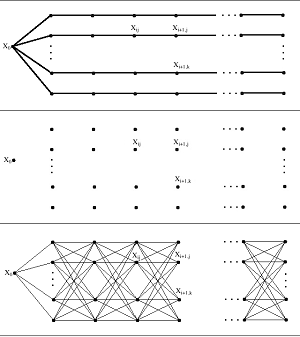
\includegraphics[width=7cm]{mesh_figure.png} 
			
		\end{center}
	\end{figure}
	\newpage
	
	
	The weights are related to the probability density function. Intuitively, given a node $(i,j)$, and according to the SDE (1), some $(k,j+1)$ are more likely to be reached by the stock path than others. An important issue of the stochastic mesh method is to determine those weights. 
	
	\subsubsection{likelihood Ratio Weights}
	
	Suppose that we want to evaluate the following $C(t_{i+1}, x) = \mathbb{E}[h(t_{i+1},X_{i+1})| X_i = x]$ conditional expectation where $h$ is smooth enough to ensure the existence. 
	Let us denote by $(f(t_i, X_i, X_{i+1}))_{i \in {1, ..., m-1}}$ the transition densities of Markov Chain $(X_i)_{i \in {1, ..., m}}$, and $g_(t_i, X_i)$ density function of $X_i$. 
	Then, by definition, 
	\begin{equation}
	\mathbb{P}[X_{i+1} \in A|X_i=x] = \int_{A}^{}f_i(x, y)dy  \notag
	\end{equation}
	
	\begin{eqnarray}
	\mathbb{E}[h(t_{i+1},X_{i+1})|X_i = x] &=& \int h(t_{i+1},y) f(t_i, x, y)dy \notag \\
	&=& \int h(t_{i+1},y)  \frac{f(t_i, x, y)}{g(t_{i+1}, y)}g(t_{i+1}, y)dy \notag \\
	&=& \mathbb{E}[h(t_{i+1},X_{i+1})  \frac{f(t_i, x, X_{i+1})}{g(t_{i+1}, X_{i+1})}]
	\end{eqnarray}
	
	Defining now 
	
	\begin{eqnarray}
	\hat{C}(t_i, X_{i,j}) &=& \frac{1}{N} \sum_{k=1}^{N} h(t_{i+1},X_{i+1}) \omega_{i,j}^k \notag \\
	\omega_{i,j}^k & = &\frac{f(t_i, X_{i, j}, X_{i+1, k})}{g(t_{i+1}, X_{i+1, j})} \notag
	\end{eqnarray} 
	
	$\widehat{C}$ is an unbiased estimator of $C$ when $N\rightarrow \infty$, with a convergence rate of $\mathcal{O}(\frac{1}{\sqrt{N}})$. 
	
	Using definition of $g$, 
	
	\begin{eqnarray}
	g(t_{i+1}, X_{i+1}=y) &=& \int f(t_i, x, y) g(t_i, x)dx \notag \\
	&=& \mathbb{E}[f(t_i, X_i, y)]
	\end{eqnarray}
	
	Finally, using a second time a Monte-Carlo estimator for the previous density function, we simulate the weights by : 
	
	\begin{equation}
	\omega_{i,j}^k =  \frac{f(t_i, X_{i, j}, X_{i+1, k})}{\frac{1}{N} \sum_{j=1}^{N}f(t_i, X_{i, j}, X_{i+1,k})} \notag
	\end{equation}
	
	
	As a reminder, our main problem is calculation of : 
	
	
	\begin{empheq}[left = \empheqlbrace]{align}
	&\mathbb{E}[Y_{i+1}|X_i]\\
	&\mathbb{E}[Y_{i+1}\Delta B_{i+1}|X_i]
	\end{empheq}
	
	So adapting our previous calculus
	
	\begin{empheq}[left = \empheqlbrace]{align}
	\widehat{Y_{i, j}} &= \frac{1}{N} \sum_{k=1}^{N} Y_{i+1} \omega_{i,j}^k\\
	\widehat{Y\Delta B}_{i, j} &= \frac{1}{N} \sum_{k=1}^{N} Y_{i+1, k}\Delta B_{i+1, j}^k \omega_{i,j}^k
	\end{empheq}
	
	are unbiased estimators of our two conditional expectations. 
	
	\subsubsection{Limits}
	
	
	Mesh Method presents two main drawbacks, especially when used in higher dimension. 
	First, computing the weights requires transition densities, which is not always available (can be computed approximatively though, using the Euler scheme, when SDE is not a geometric Brownian motion). 
	Second, its time complexity of $\bigO(dmN^2)$, where $d$ is the dimension, $m$ the number of steps used for discretization, and $N$ the number of samples, limits the use of big samples especially. 
	For instance, $10^4$ particles would require in Python 10GB of memory in dimension four. Indeed, one float takes 24 bytes in memory, so generating $10^4$ particles requires at every step the construction of an $N\times N$ matrix of weights, taking then $24\times N^2 = 2.4.10^9$ bytes in memory. Adding the 4-dimension, we reach the 10GB memory ... 
	
	\subsection{Least Square Monte-Carlo}
	
	A Least Square Monte-Carlo can be used for the simulation of conditional expectation of the form $\mathbb{E}[Y|X]$, when $X$ and $Y$ are square integrable random variables, and a set of numerical values $(X,Y)$ is available. 
	
	Longstaff and Schwartz made this method popular in financial mathematics for the pricing of American Options, which is build upon a basis projection, i.e upon the statement $\mathbb{E}[Y|X] = h(X)$. 
	
	$h$ minimizes what we call a least square function, i.e. 
	
	\begin{equation}
	h = \arg \min\{\mathbb{E}[|Y - f(X)|^2] \quad,  \text{f s.t} \quad \mathbb{E}[|f(X)|^2]<\infty\}
	\end{equation}
	
	This infinite-dimensional problem can be restricted to smaller set of functions to look for. 
	Our simulations for one asset will be using polynomials. 
	Indeed, we have decided not to use this method in bigger dimension as projections on multi-polynomials requires too much computational time. 
	
	
	\subsection{Random Forest and Tree Based regression}
	
	Random Forest ranks among the most popular machine learning methods, as it provides the user simplicity and accuracy. 
	For more details about time complexity and hyperparameters explanations, the reader can refer to Appendix A, which analyses more exhaustively an example of regression on housing market data in Iowa (\cite{kaggle:housing}). 
	
	We will focus here on how Random Forest regreesion can be used to approximate the conditional expectations needed for solving our BSDE problem. 
	
	
	\subsubsection{Random Forest}
	
	
	
	
	\subsection{Gradient Boosting}
	
	
	\subsection{Derivative}
	
	Another method we will use in the simulations is the derivative one. 
	As explained in 1-BSDE section, $(Y_t = u(t;X_t);Z_t =\sigma(t,x)^T D_xu(t;X_t))$ is solution to (8), with $u$ solution to semi-linear PDE (9).  
	Given our algorithm process
	
	\begin{algorithm}
		\caption{BSDE Algorithm}
		\label{algo:derivative1}
		\begin{algorithmic}[1]
			\Procedure{BSDE}{}
			\For{$t \in \{T-1, 0\}$}
			\State $Z[t] =\frac{1}{\Delta t}\mathbb{E}_t[Y_{t + 1} \Delta B_t]$
			\State $Y[t] = \mathbb{E}_t[Y_{t+1} +  f(t,X_t, Y_{t+1}, Z_t)\Delta t]$
			\EndFor
			\EndProcedure
		\end{algorithmic}
	\end{algorithm}
	
	for all $t$ we can compute once the previous algorithm, and enhance it by taking $Y_t = \phi(t, X_t)$ with $\phi$ smooth enough to be derivable, and derive from there $Z_t = \nabla \phi (t, X_t)$. Hence
	
	\begin{algorithm}
		\caption{BSDE Algorithm}
		\label{algo:derivative2}
		\begin{algorithmic}[1]
			\Procedure{BSDE}{}
			\For{$t \in \{T-1, 0\}$}
			\State $Z[t] =\frac{1}{\Delta t}\mathbb{E}_t[Y_{t + 1} \Delta B_t]$ \text{by RandomForest for instance}
			\State $Y[t] = \mathbb{E}_t[Y_{t+1} +  f(t,X_t, Y_{t+1}, Z_t)\Delta t]$
			\For {\_\_ = 1:M}
			\State  \text{Get $\phi$ such that} $Y_t \sim \phi(t, X_t)$
			\State  $Y_{new} = \phi(t, X_t)$
			\State 	$Z_{new} = \nabla \phi(t, X_t)$ \text{gives a new smoother $Z$}
			\State  $Y[t] = \mathbb{E}_t[Y_{t+1} +  f(t,X_t, Y_{t+1}, Z_{new})\Delta t]$
			\EndFor
			\EndFor
			\EndProcedure
		\end{algorithmic}
	\end{algorithm}
	
	$Z$ being a very noisy process, due to the factor $\frac{1}{\Delta B_t\Delta t}$, especially when $\Delta t \rightarrow 0$, it seemed relevant to get the smoothest approximation possible. 
	
	In our simulation, we use a kernel regression to recover a smooth $\phi$ function. 
	Kernel regression consists on a sum of smooth functions, each one giving an approximation around a point $(X_i, Y_i)$. 
	
	Denoting $K(\frac{X - X_i}{l})$ the kernel function for the point $(X_i, Y_i)$, where l controls the scale and length,  we define the weight $\omega(X, X_i) = \frac{K(\frac{X - X_i}{l})}{\sum_{i=1}^{N} K(\frac{X - X_i}{l})}$ such that $\phi(X) = \sum_{i=1}^{N} \omega(X, X_i)Y_i$. 
	
	\begin{Ex}
		Let $Y$ be a random variable defined by $Y = \sin()$
	\end{Ex}
	
	\subsection{Picard Iteration}
	
	The noisy $Z_t$ process can be approximated iteratively using a Picard iteration. This idea has been inspired from E.Gobet \cite{gobet:picard}. 
	
	This iteration takes its origin from Picard's convergence theorem 
	
	\begin{Th}
		
	\end{Th}
	
	
	\subsection{Variance Reduction}	
	
	
	\newpage 
	
	\section{Applications}
	
	\subsection{Introduction}
	
	The following simulations are computed on Python 3.5, with available forty-eight CPU available in the Department of Applied Probability and Statics of NUS. 
	
	Each example relies on a theoretical solution, or a comparison found in BSDE literature. 
	
	We will give for every example the solution given by the previous cited methods, with its $95\%$ confidence interval, and the average time. 
	When not specified, we run \#20 simulations for every average given, and use a Picard iteration number of three. 
	
	We apply BSDE theory on European and American option pricing, respectively on one and multiple assets.
	
	First example analysis will be exhaustive, especially comparison of  different methods implemented for regression step.
	Then, we give multiple results obtained on other examples from literature, detailing time computation and accuracy.   
	
	
	\subsubsection{Bid-ask model}
	
	Suppose the dynamic of the underlying assets to be : 
	
	\begin{eqnarray}
	\frac{dS_t^i}{S_t^i}=\mu^i dt + \sigma^i dB_t^i\\
	<dB_t^i,dB_t^j> = 1 \quad \text{if} \quad i=j
	\end{eqnarray}
	
	and let the agent be able to lend ($r$) and borrow ($R$) money using two market accounts : 
	
	\begin{equation}
	\left\{
	\begin{aligned}
	d\alpha_t &= R \alpha_t dt\\
	d\beta_t &= r \beta_t dt\\
	\end{aligned}
	\right.
	\end{equation}
	
	Let $Y_t$ be the portfolio value at time $t$. 
	
	\begin{displaymath}
	dY_t = \sum_{i = 1}^{p} \Phi^i_t \frac{dS^i_t}{S^i_t} + (Y_t - \sum_{i = 1}^{p} \Phi^i_t)^+rdt - (Y_t - \sum_{i = 1}^{p} \Phi^i_t)^-Rdt
	\end{displaymath}
	
	where $\Phi^i_t$ represents the amount of shares invested in stock $S_t^i$ at time $t$.
	
	We get then the following BSDE : 
	
	\begin{equation}
	-dY_t = f(t,Y_t,Z_t)dt - Z_tdW_t  
	\end{equation}
	
	where 
	
	\[
	\left\{
	\begin{aligned}
	f(t,Y_t,Z_t) & =   Z_t.\theta - r.Y + (R-r)(Y- \sum_{i=1}^{d}(\sigma^{-1}Z_t)_i)^-\\
	Z_t & = \sigma. \Phi_t\\
	\theta &= \sigma^{-1}(\mu - r)\mathbbm{1}
	\end{aligned}
	\right.
	\]
	
	
	\subsubsection{Credit Valuation Adjustment (CVA)}
	
	Using same notations than \cite{GuyonLabordere:cva}, CVA can be transformed into a BSDE problem :
	\begin{displaymath}
	\left\{
	\begin{aligned}
	-dY_t& = f(t,Y_t,Z_t)dt - Z_tdW_t \\
	f(t,Y_t,Z_t) & =  \beta (Y_t^+ - Y_t)
	\end{aligned}
	\right.
	\end{displaymath}
	
	with the corresponding semi-linear PDE 
	
	\begin{eqnarray}
	\partial_t u + \mathcal{L}u + \beta(u^+ -u) &=& 0 \notag \\
	u(T, x) &=& g(x) \notag
	\end{eqnarray}
	
	where $\mathcal{L}$ is the Itô generator of a diffusion $X_t$
	
	There is no process $Z$ to regress here, but we will analyse how Random Forest performs on $\E_t[Y_{t+ \Delta t}^+]$ 
	
	
	
	\subsection{One dimension}
	
	\subsubsection{Bid-ask European call option}
	\newpage 
	
	Referring to Gobet, Lemor and Warin's simulations in \cite{gobet:example}, we take the following numerical values $X_0 = 100.$, $K=100$, $\sigma=0.2$, $r=0.04$, $R=0.06$, $\mu = 0.06$ and $q = 0.$. 
	
	We compute the pricing of the European call (i.e payoff $(X_T - K)^+$) on a single asset associated. This problem has a theoretical solution, given by the Black-Scholes model with $R$ used as free-risk rate. 
	Indeed, to hedge himself, the financial seller will borrow money to buy assets, hence the use of $R$. 
	
	
	
	
	
	Specifically to each method, table \eqref{table:bid_ask_european_call_1D} draws the mean on run, with its 95\% confidence interval and the time average of one run. 
	\begin{table}[H]
		\centering
		\caption{Bid-ask European call option with one asset}\label{table:bid_ask_european_call_1D}
		\rowcolors{5}{}{gray!10}
		\begin{tabular}{*5c}
			\toprule
			& \multicolumn{3}{c}{European Call} \\
			\cmidrule(lr){2-5}
			Method & Random Forest  & Least-Square & Mesh & Derivative \\    
			& $(200, 700)$ & degree = $6$     & $N = 4 000$ &  $N = 4 000$ \\
			& N = 10.000 & N = 100.000     &  &  l= 1.0\\
			\midrule
			mean &     7.142   & 7.155  &  7.188  &  7.178 \\ 
			95\% confidence interval &   $[7.134, 7.150]$     &    $[7.152, 7.159]$     & $[7.174, 7.201]$ & $[7.148, 7.208]$  \\
			time average for on run &        &  &  &  \\
			\bottomrule
		\end{tabular}
	\end{table}
	
	
	\subsubsection{Bid-ask European call combination}
	
	Once again, we take an example from Gobet, Lemor and Warin's 's article \cite{gobet:example}, where we consider still two different rates (bid-ask model). This time, the differences $R-r$ and $\mu - r$ are larger, as $\mu = 0.05$, $r=0.01$ and $R=0.06$. This emphasizes the role of the noisy process $Z$ during the regression steps. 
	We keep working with a 20\% volatility $\sigma=0.02$, no dividend yield $q=0$, and an initial asset value $X_0 = 100$. We consider, following Gobet's example a call combination derivative, i.e with payoff $(X_T - K_1)^+ - 2(X_T - K_2)^+$, with $K_1 = 95$ and $K_2 = 105$.
	
	In their simulations, Gobet, Lemor and Warin's use projections on function basis to approximate the conditional expectations. They make use of hypercubes partitions, Voronoi partitions (VP) and global polynomials. 
	
	There is no theoretical price for this example, as the non-linearity of driver has a real impact. The option buyer has to alternatively to borrow and lend money to hedge his position.
	
	However, a simulation price given by Hypercubes and VP seem to converge to 2.95, which will take as reference. 
	Applying our derivative, stochastic mesh, LSM and Random Forest methods to this example, we get
	
	\begin{table}[!h]
		\centering
		\caption{Bid-ask European call combination option with one asset}\label{table:bid_ask_call_combi_1D}
		\rowcolors{5}{}{gray!10}
		\begin{tabular}{*5c}
			\toprule
			& \multicolumn{3}{c}{Call combination } \\
			\cmidrule(lr){2-5}
			Method & Random Forest  & Least-Square & Mesh & Derivative \\    
			& $(200, 700)$ & degree = $6$     & $N = 4 000$ &  $N = 4 000$ \\
			& N = 10.000 & N = 100.000     &  &  l= 1.0\\
			\midrule
			mean &     2.969   & 2.938  &  2.841  &  2.940 \\ 
			95\% confidence interval &   $[2.965, 2.974]$     &    $[2.937, 2.940]$     & $[2.834, 2.848]$ & $[2.912, 2.969]$  \\
			time average &        &  &  &  \\
			\bottomrule
		\end{tabular}
	\end{table}
	
	
	\subsubsection{CVA}
	
	\begin{table}[H]
		\centering
		\caption{CVA}\label{table:CVA}
		\rowcolors{5}{}{gray!10}
		\begin{tabular}{*5c}
			\toprule
			& \multicolumn{3}{c}{CVA} \\
			\cmidrule(lr){2-4}
			Method & Random Forest  & Least-Square & Mesh & Derivative \\    
			& $(200, 700)$ & degree = $6$     & $N = 4 000$ &  $N = 4 000$ \\
			\midrule
			mean &        &  &       \\ 
			95\% confidence interval &        &        &  \\
			time average &        &  &  \\
			\bottomrule
		\end{tabular}
	\end{table}
	
	
	\subsubsection{American Option}
	
	
	\begin{table}[H]
		\centering
		\caption{One dimensional American Option}\label{table:amoption}
		\rowcolors{5}{}{gray!10}
		\begin{tabular}{*5c}
			\toprule
			& \multicolumn{3}{c}{American Option 1D} \\
			\cmidrule(lr){2-4}
			Method & Random Forest  & Least-Square & Mesh & Derivative \\    
			& $(200, 700)$ & degree = $6$     & $N = 4 000$ &  $N = 4 000$ \\
			\midrule
			mean &        &  &       \\ 
			95\% confidence interval &        &        &  \\
			min &        &  &  \\
			max &  &        &        \\
			\bottomrule
		\end{tabular}
	\end{table}
	
	
	\subsection{High Dimension}
	
	\subsubsection{Geometrical average on seven assets following bid-ask model}
	
	After managing to tune our Random Forest hyperparameters in one dimension cases, we now turn to more sophisticated problems. 
	First case which drew our attention is the pricing of a Geometrical Average call option on seven assets. This derivative has a payoff $((\prod_{i=1}^{7}X_T^{(i)})^{\frac{1}{7}} - K)^+$. 
	Taking seven independent assets in Black-Scholes model, this problem is equivalent to taking a one dimensional European call. 
	
	Indeed, let us assume $\forall i \in \{1, \cdots, d\}$, $X_T^{i} = X_0^{i} \exp^{(r - \frac{\sigma^2}{2})T + \sigma B_T^{i}}$. 
	Then 
	
	\begin{align}
	(\prod_{i=1}^{7}X_T^{(i)})^{\frac{1}{d}} &= X_0 \exp^{(r - \frac{\sigma^2}{2})T + \frac{\sigma}{d}\sum_{i=1}^{d}B_T^{i}} \notag \\
	&\overset{\mathcal{L}}{\sim} X_0 \exp^{(r - \frac{\sigma^2}{2})T + \frac{\sigma}{d}\sum_{i=1}^{d}\mathcal{N}(0, T)} \notag \\
	&\overset{\mathcal{L}}{\sim} X_0 \exp^{(r - \frac{\sigma^2}{2})T + \frac{\sigma}{d}\mathcal{N}(0, dT)} \notag \\
	&\overset{\mathcal{L}}{\sim} X_0 \exp^{(r - \frac{\sigma^2}{2})T + \frac{\sigma}{\sqrt{d}}\mathcal{N}(0, T)} \notag
	\end{align}
	
	Taking 
	
	\begin{align}
	\tilde{r} - \frac{\tilde{\sigma}^2}{2} = r - \frac{\sigma^2}{2} \\
	\tilde{\sigma} = \frac{\sigma}{\sqrt{d}}
	\end{align}
	
	\begin{align}
	\tilde{r} = r + \frac{\sigma^2}{2}\frac{d-1}{d} \\
	\tilde{\sigma} = \frac{\sigma}{\sqrt{d}}
	\end{align}
	
	\begin{displaymath}
	(\prod_{i=1}^{7}X_T^{(i)})^{\frac{1}{d}} \overset{\mathcal{L}}{\sim} X_0 \exp^{(\tilde{r} - \frac{\tilde{\sigma}^2}{2})T + \tilde{\sigma}\mathcal{N}(0, T)}
	\end{displaymath}
	
	Hence, a theoretical price is given by usual Black-Scholes formula, $Y_0 = BS(T, K, X_0, \tilde{r}, \tilde{sigma}) = 3.301$
	
	\begin{table}[!h]
		\centering
		\caption{Bid-ask  Geometric Average European Call option on 7 assets}\label{table:call7D}
		\rowcolors{5}{}{gray!10}
		\begin{tabular}{*5c}
			\toprule
			& \multicolumn{3}{c}{Geometric Average European Call} \\
			\cmidrule(lr){2-5}
			Method & Random Forest  & GradBoosting & Mesh & Derivative \\    
			& $(200, 700)$ &     & $N = 4 000$ &  $N = 4 000$ \\
			& N = 10.000 & N = 10.000     &  &  l= 1.0\\
			\midrule
			mean &     3.299   &   &  3.318  &  3.330 \\ 
			95\% confidence interval &   $[3.296, 3.304]$     &         & $[3.310, 3.327]$ & $[3.260, 3.401]$  \\
			time average &        &  &  &  \\
			\bottomrule
		\end{tabular}
	\end{table}
	
	\subsubsection{Geometrical average on twenty-five assets following bid-ask European call model}
	
	\begin{table}[H]
		\centering
		\caption{Bid-ask European call option with one asset}\label{table:1}
		\rowcolors{5}{}{gray!10}
		\begin{tabular}{*5c}
			\toprule
			& \multicolumn{3}{c}{Methods tested} \\
			\cmidrule(lr){2-4}
			Method & Random Forest  & Least-Square & Mesh & Derivative \\    
			& $(200, 700)$ & degree = $6$     & $N = 4 000$ &  $N = 4 000$ \\
			\midrule
			mean &     7.142   &  &       \\ 
			95\% confidence interval &        &        & CHECK \\
			time average &        & CHECK & CHECK \\
			\bottomrule
		\end{tabular}
	\end{table}
	
	\subsubsection{Geometrical average on twenty assets following bid-ask European call combination model}
	
	\begin{table}[!h]
		\centering
		\caption{Bid-ask European call option with one asset}\label{table:1}
		\rowcolors{5}{}{gray!10}
		\begin{tabular}{*5c}
			\toprule
			& \multicolumn{3}{c}{Methods tested} \\
			\cmidrule(lr){2-4}
			Method & Random Forest  & Least-Square & Mesh & Derivative \\    
			& $(200, 700)$ & degree = $6$     & $N = 4 000$ &  $N = 4 000$ \\
			\midrule
			mean &     7.142   &  &       \\ 
			95\% confidence interval &        &        & CHECK \\
			min &        & CHECK & CHECK \\
			max & CHECK &        &        \\
			\bottomrule
		\end{tabular}
	\end{table}
	
	\subsubsection{Exchange Option between two correlated assets}
	
	\begin{table}[!h]
		\centering
		\caption{Bid-ask European call option with one asset}\label{table:1}
		\rowcolors{5}{}{gray!10}
		\begin{tabular}{*5c}
			\toprule
			& \multicolumn{3}{c}{Methods tested} \\
			\cmidrule(lr){2-4}
			Method & Random Forest  & Least-Square & Mesh & Derivative \\    
			& $(200, 700)$ & degree = $6$     & $N = 4 000$ &  $N = 4 000$ \\
			\midrule
			mean &     7.142   &  &       \\ 
			95\% confidence interval &        &        & CHECK \\
			min &        & CHECK & CHECK \\
			max & CHECK &        &        \\
			\bottomrule
		\end{tabular}
	\end{table}
	
	\subsubsection{Exchange Option between the average of twenty correlated assets}
	
	\begin{table}[!h]
		\centering
		\caption{Bid-ask European call option with one asset}\label{table:1}
		\rowcolors{5}{}{gray!10}
		\begin{tabular}{*5c}
			\toprule
			& \multicolumn{3}{c}{Methods tested} \\
			\cmidrule(lr){2-4}
			Method & Random Forest  & Least-Square & Mesh & Derivative \\    
			& $(200, 700)$ & degree = $6$     & $N = 4 000$ &  $N = 4 000$ \\
			\midrule
			mean &     7.142   &  &       \\ 
			95\% confidence interval &        &        & CHECK \\
			min &        & CHECK & CHECK \\
			max & CHECK &        &        \\
			\bottomrule
		\end{tabular}
	\end{table}
	
	\newpage
	
	
	
	\section{Second Order BSDE}
	
	This section presents an extension to 1-BSDE models, with a direct application on non-linear PDE.
	Cheridito, Soner, Touzi and Victoir \cite{cheridito:2BSDE} introduced the notion of Second Order BSDEs (2-BSDEs).
	\newline
	We will give a quick definition of the problem, before explaining the link with non-linear PDE. We will finish with an example of discretization for this type of BSDE. 
	For a larger review of the theory of 2-BSDEs, we refer to Soner, Touzi and Zhang \cite{touzi:2BSDE}.
	
	\subsection{Definition}
	
	We now introduce second
	order BSDEs for which the corresponding PDE can be non-linear in the second
	order derivatives and are therefore connected to HJB equations with a control on the diffusion coefficient. Examples of such HJB equations include the
	Black-Scholes-Barenblatt equation.
	The following definition is given by \cite{cheridito:2BSDE}
	
	\begin{defn}
		Let $(s, x) \in \left[0, T\right) \times\R^d$ and $(Y_t, Z_t, \Gamma_t, \alpha_t)_{t\in [0, T]}$ be a quadruple of $(\mathcal{F}_t)$-adapted processes taking values in $\R$, $\R^d$, $\mathcal{S}^d$ \footnote{Space of symmetrical matrices with dimension}, and $\R^d$ respectively. We call $(Y, Z, \Gamma, \alpha)$ a solution to a 2-BSDE corresponding to $(X^{s,x}, f, g)$ \footnote{$X_s = x$} if
		
		\begin{align} \label{2-BSDE}
		dY_t &= - f(t,X_t^{s,x}, Y_t,Z_t, \Gamma_t)dt + Z_t' \diamond dX_t^{s,x} \quad t\in [s, T)\\
		dZ_t &= \alpha_tdt + \Gamma_t dX_t^{s,x} \quad t\in [s, T) \notag\\
		Y_T & = g(X_T^{s,x}) \notag
		\end{align}
		where $\diamond$ represents the Stratanovich integral, related to Itô integration by 
		
		\begin{align}
		Z_t' \diamond dX_t^{s,x} &= Z_t' dX_t^{s,x} + \frac{1}{2}d\langle Z, X_t^{s,x}\rangle_t \notag \\
		&= Z_t' dX_t^{s,x} + \frac{1}{2}Tr\left[\Gamma_t d\langle X_t^{s,x}, X_t^{s,x}\rangle_t \right] \notag \\
		& = Z_t' dX_t^{s,x} + \frac{1}{2}Tr\left[\Gamma_t \sigma(t, X_t^{s,x})\sigma(t, X_t^{s,x})' \right]dt \notag
		\end{align}
		
	\end{defn}
	
	\subsection{Existence and Uniqueness}
	
	The reader can refer to "Wellposedness of Second Order Backward SDEs" \cite{touzi:2BSDE} article which provides an existence and uniqueness theory. 
	
	\subsection{Second order BSDE and non-linear PDE}
	
	Let us consider the non-linear PDE 
	\begin{equation}\label{eq:nonlinearpde}
	\partial_t u + \mathcal{L}u + f(t, x, u, D_xu(t,x), D^2_xu(t,x)) = 0, \quad (t,x)\in [0, T) \times \mathbb{R}^d
	\end{equation}
	with the terminal condition $u(T; x) = g(x)$ and $\mathcal{L}$ the Itô generator of $X$.
	Such an equation appears when we consider a stochastic control problem
	with no control on the diffusion coefficient. 
	($Y_t = u(t;X_t)$ , $Z_t =D_xu(t;X_t)$, $\Gamma_t = D^2_xu(t;X_t)$, $\alpha_t = (\partial_t + \mathcal{L})D_xu(t,X_t)$) is a solution to the 2-BSDE under some assumptions
	
	\begin{Prop}
		Generalization of Feynman-Kac's formula : \newline
		Let $u$ be a function of $\mathcal{C}^{1,2}$ satisfying (\ref{eq:nonlinearpde}) and suppose that there exists a
		constant $C$ such that, for each $(t; x) \in [0; T] \times \mathbb{R}^d$
		\begin{equation}
		|\sigma(t,x)^T D_xu(t;X_t)|\leq C(1 + |x|)
		\end{equation}
		Then $(Y_t = u(t;X_t);Z_t = D_xu(t;X_t), \Gamma_t = D^2_xu(t,x))$ is the unique solution to 2-
		BSDE (\ref{2-BSDE}).
	\end{Prop} 
	
	
	\subsection{Discretization}
	
	Using the previous tricks (multiplying by $dB_t$ in $dZ_t$ expressions and using measurability properties) gives us the following discretization for the 2-BSDE : 
	
	\begin{align}
	Y_{t_n} &= g(X_{t_n}) \notag \\
	Z_{t_n} &= Dg(X_{t_n}) \notag \\
	\Gamma_{t_i} &= \frac{1}{\Delta t_i}\mathbb{E}[Z_{t_{i + 1}} \Delta B_{t_i}^T  | \mathcal{F}_{t_i}]\sigma(t_i, X_{t_i})^{-1} \notag \\
	Z_{t_i} &= \sigma(t_i, X_{t_i})'^{-1}\frac{1}{\Delta t_i}\mathbb{E}[Y_{t_{i + 1}} \Delta B_{t_i}  | \mathcal{F}_{t_i}] \notag 
	\end{align}
	
	
	
	\begin{displaymath}
	Y_{t_i} = \mathbb{E}[Y_{t_{i + 1}} | \mathcal{F}_{t_i}] +  (f(t_i,S_{t_i}, Y_{t_{i + 1}}, Z_{t_i}, \Gamma_{t_i}) - \mathtt{tr}[\sigma(t_i, X_{t_i}) \sigma(t_i, X_{t_i})'\Gamma_{t_i}])\Delta t_i
	\end{displaymath}
	
	
	Given $Y_{t_n}$ we can get $Y_0$ using the previous discretization backwardly. 
	
	\subsection{Application : Portfolio Optimization}
	
	Arash Fahim, Nizar Touzi and Xavier Warin analysed an example of 2-BSDE, the continuous-time portfolio optimization in financial mathematics (\cite{touzi:2bsdesimulation}). 
	Two dimensional and Five dimensional examples are analysed, and we will run a Random Forest Regression on both examples, and will draw a comparison. 
	
	\newpage 
	
	
	\section{Conclusion}
	
	After reviewing theory of BSDE, we gave here several regression methods to compute conditional expectation appearing in the backward process. 
	Relying on existent methods found in literature, such as Stochastic Mesh by Broadie and Glasserman \cite{glasserman:broadie} and Least Square \cite{bender:lsmbsde}, we computed different approaches, Random Forest, Gradient Boosting, and Derivative, for comparison purposes.
	We focused on accuracy (i.e mean and variance), and time analysis to draw simulation conclusions. 
	
	
	Applying these on several examples leads to multiple conclusions. 
	
	First, dealing
	
	\newpage
	\begin{appendices}
		\section{Random Forest}
		
		
		\begin{minipage}{\textwidth-2\fboxrule-2\fboxsep\relax}
			The following section is the main contribution to BSDE analysis, as it uses a machine learning method, Random Forest (Randomized Tree Decision), for the regression step. 
			We will first focus on a quick analysis of decision trees. From there, we will explain Randomized Trees methods using a housing market data in Iowa. We will mainly focus on  hyperparameters tuning and complexity of the different Random Trees methods. 
		\end{minipage}
		
		
		\subsection{Decision Tree}
		Machine learning research has given plenty of new methods for classification and regression problems. Most effective remain the tree based methods, intuitive and reliable for almost any kind of data. 
		
		We use Gilles Louppe (here) 's notations : 
		
		\begin{defn}
			A tree is a graph $G = (V, E)$ in which any two vertices (or
			nodes) are connected by exactly one path.
		\end{defn}
		
		\begin{defn}
			A rooted tree is a tree in which one of the nodes has been
			designated as the root. In our case, we additionally assume that a rooted tree
			is a directed graph, where all edges are directed away from the root.
		\end{defn}
		
		\begin{defn}
			If there exists an edge from t1 to t2 (i.e., if (t1, t2) 2 E)
			then node t1 is said to be the parent of node t2 while node t2 is said to be a
			child of node t1.
		\end{defn}
		
		\begin{defn}
			In a rooted tree, a node is said to be internal if it has one
			or more children and terminal if it has no children. Terminal nodes are also
			known as leaves.
		\end{defn}
		
		\begin{defn}
			A binary tree is a rooted tree where all internal nodes have
			exactly two children.
		\end{defn}
		
		
		\newpage 
		\begin{figure}[t!]
			\centering
			\begin{subfigure}[t]{0.3\textwidth}
				\includegraphics[width=\textwidth]{decision_tree.png}
				\caption{}
				\label{fig:gull1} %  
			\end{subfigure}
			~~~~~~~~~~~~~~~
			\begin{subfigure}[t]{0.3\textwidth}
				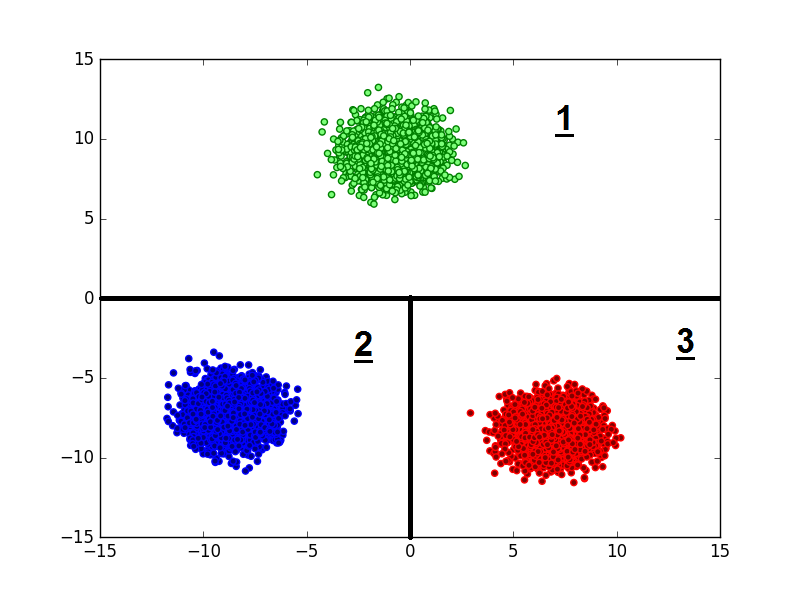
\includegraphics[width=\textwidth]{classification_presentation.png}
				\caption{}
				\label{fig:gull}
			\end{subfigure}
			\caption{A decision tree built for a classification $(1, 2, 3)$ problem from an input space $[-15, 15] \times [-15, 25]$}
		\end{figure}
		
		
		\subsection{Randomized Forest}
		
		From Decision trees, we get low bias and high variance. To overcome this issue, generating random decision trees (i.e random initial state of the tree, random features, ...) and averaging over them makes it possible to get better bias-variance results. 
		The theoretical properties and statistical mechanisms that drive the algorithm are still not clearly and entirely understood.
		Random forests indeed evolved from empirical successes rather
		than from a sound theory. As such, various parts of the algorithm remain heuristic rather than theoretically motivated. 
		
		We will mainly focus on empirical results 
		
		
		\subsection{Complexity}
		
		Let us consider p predictor variables $(x_1, \cdots, x_p) \in D \subset \R^p$  of a response variable $y$. The goal of this subsection is to determine the time complexity of the Random Forest model, given $N$ samples data. 
		\newline
		Let $T(N)$ denote the time for building one decision tree. 
		
		\begin{figure}[h!]
			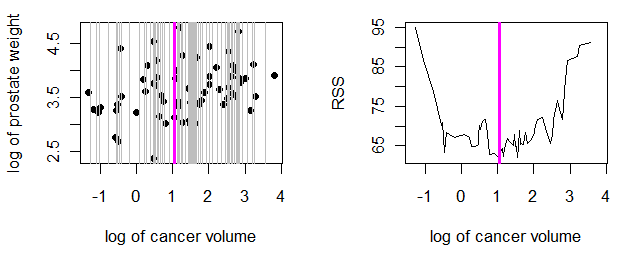
\includegraphics[scale=0.8]{time_complexity/sorting_split.png}
			\caption{Choosing the best vertical split using RSS measure} \label{figure:sorting}
		\end{figure}
		
		
		$T(N)$ can be approximated recursively. 
		Indeed, we can grow a decision tree in three steps : find the best splitting, grow a left child tree, and grow a right child tree.
		\newline 
		Let us denote the time complexity of these steps by $s(N)$, $T_{left}(N)$ and $T_{right}(N)$ respectively. 
		Hence : $T(N) = s(N) + T_{left}(N) + T_{right}(N)$.
		We will present both best case and worst case complexity for every step, and we will assume the time complexity to lay in between. 
		\paragraph{splitting and partitioning}
		The partitioning step requires at least an iteration over the N samples, so we can already set a linear lower bound on the time complexity within a node.
		Finding a split can be done using Figure \ref{figure:sorting} (example from \cite{Cutler:slides}) method, i.e computing a Residual Sum of Squares (RSS) and minimize it. 
		This operation requires to sort the N samples for every predictor $x_i, i\in \{1, \cdots, p\}$. 
		Time complexity to sort a list with size $N$ is at worst $\mathcal{O} (N)$, and at best $\bigO(\log N)$. 
		Combining both splitting and partitioning, time complexity is at worst $\mathcal{O} (p N^2)$ and at best $\bigO(p N \log N)$ . 
		Random Forest can limit the search over $K \leq p$ features, which reduces this complexity between $\mathcal{O} (K N\log N)$ and $\mathcal{O} (K N^2)$. 
		
		\paragraph{Child left and right trees}
		
		The best case for growing these two child trees is intuitively $\frac{N}{2}$. The worst case would be having a tree with one pure leaf	and $N - 1$ samples in the other tree. 
		
		Hence, 
		\begin{displaymath}
		s(N) + T_{left}(\frac{N}{2}) + T_{right}(\frac{N}{2}) \leq T(N) \leq s(N) + T_{left}(1) + T_{right}(N - 1) 
		\end{displaymath}
		Or
		
		\begin{displaymath}
		s(N) + 2.T(\frac{N}{2})\leq T(N) \leq s(N) + T(1) + T(N - 1) 
		\end{displaymath}
		
		
		Having a recurrence equation, let us make use of the following theorem. 
		
		\begin{Th}\label{theorem:master}Master Theorem
			
			$$T(n) = \left\{ \begin{array}{ll}
			c             & \mbox{if $n < d$,}\\
			aT(n/b) + f(n)& \mbox{if $n \geq d$},
			\end{array}
			\right. $$
			where $a \geq 1, b > 1,$ and $d$ are integers and $c$ is a positive
			constant.  Let $\nu = \log_b a$.
			\begin{description}
				\item[Case (i) $f(n)$ is ``definitely smaller'' than $n^\nu$:] If there is a small contant $\epsilon > 0,$ such that 
				$f(n) \preceq n^{\nu - \epsilon}$, that is,
				$f(n) \prec n^\nu$, then $T(n) \sim n^\nu$.
				
				\item[Case (ii) $f(n)$ is ``similar in size'' to $n^\nu$:] If there is a constant $k \geq 0$, such that 
				$f(n) \sim n^{\nu}( \log n)^k$, then 
				$T(n) \sim n^{\nu}(\log n)^{k+1}$.
				
				\item[Case (iii) $f(n)$ is ``definitely larger'' than $n^\nu$:] If there are small constants $\epsilon > 0$ and $\delta < 1$, such
				that $f(n) \succeq n^{\nu + \epsilon}$ and $a f(n/b) \leq \delta
				f(n),$ for $n \geq d$, then $T(n) \sim f(n)$.
				
			\end{description}
		\end{Th}
		
		\vspace{0.5cm}
		\begin{Lemma}
			For $\frac{s(N)}{K} = \mathcal{O} (N\log N)$ and $T(N) = 2.T(\frac{N}{2}) + s(N)$, 
			time complexity for building a decision tree is $T(N) \sim K.N.\log^2N$.
		\end{Lemma}
		
		\begin{proof}
			Apply Theorem \ref{theorem:master} with $a=b=2$, $d=1$, $k=1$ and $T(N) \equiv \frac{T(N)}{K}$
		\end{proof}
		
		
		\begin{Lemma}
			For $\frac{s(N)}{K} = \mathcal{O} (N\log N)$ and $T(N) = s(N) + T(1) + T(N - 1) $, time complexity for building a decision tree is $T(N) \sim K.N.\log^2N$ (upper bound) and $T(N) $.
		\end{Lemma}
		
		\begin{proof}
			Let us rewrite in a first time the expression of $T(N)$ in a better form to make use of Theorem \ref{theorem:master}. 
			
			\begin{displaymath}
			\frac{s(N)}{K} = \mathcal{O} (N\log N)
			\end{displaymath}
			
			Let us assume there exists $C_1$, $C_2$ such that $C_1 N\log N \leq \frac{s(N)}{K} \leq C_2 N\log N$. 
			Hence, using the right side, 
			
			\begin{align}
			\frac{T(N)}{K}	& = \frac{s(N)}{K} + \frac{T(1)}{K} + \frac{T(N - 1)}{K} \notag \\
			& \leq C_2 N\log N + \frac{T(1)}{K} + \frac{T(N - 1)}{K}\notag
			\end{align}
			
			Let $t(N) = \frac{T(N)}{K}$. 
			
			\begin{align}
			& t(N) \leq C_2 N\log N + t(1) + t(N-1)\notag \\
			\iff &  t(N) - t(N-1) \leq C_2 N\log N + t(1) \notag\\
			\Rightarrow & \sum_{j=2}^{N}  t(j) - t(j-1) \leq (N-1)t(1) + C_2\sum_{j=2}^{N}j \log j \notag\\
			\Rightarrow & t(N) \leq Nt(1) + C_2\log N \sum_{j=1}^{N}j \notag\\
			\Rightarrow & t(N) \leq Nt(1) + C_2\log N \frac{N(N +1)}{2}\notag \\
			\Rightarrow & t(N) = \bigO (N^2 \log N) \notag \\
			\Rightarrow & T(N) = \bigO (KN^2 \log N) \notag
			\end{align}
			
			Similarly, using the left side gives a lower bound 
			
			\begin{align}
			& t(N) \geq C_1 N\log N + t(1) + t(N-1)\notag \\
			\iff &  t(N) - t(N-1) \geq C_1 N\log N + t(1) \notag\\
			\Rightarrow & \sum_{j=2}^{N}  t(j) - t(j-1) \geq (N-1)t(1) + C_1\sum_{j=2}^{N}j \log j \notag\\
			\Rightarrow & t(N) \geq N t(1) + C_1 \sum_{j=2}^{N}j \notag\\
			\Rightarrow & t(N) \geq Nt(1) + C_1 (\frac{N(N +1)}{2} - 1)\notag \\
			\Rightarrow & t(N) \succeq N^2 \notag \\
			\Rightarrow & T(N) \succeq N^2 \notag
			\end{align}
			
		\end{proof}
		
		Finally, growing $n_{trees}$ random trees has in the best case a time complexity $\Theta(n_{trees}KN\log^2 N)$ and in the worst case $\bigO (n_{trees} K N^2 \log N)$.
		
		\paragraph{Prediction time complexity}
		
		Iterating over every tree generated by the Random Forest, predicting depends on the depth of the tree. 
		Similarly to previous analysis, we can lower bound and upper bound the depth of one tree. 
		Indeed, let $D(N)$ denote the depth of a tree generated in the Forest. 
		
		\begin{itemize}
			\item 
			Best case is again a $\frac{N_{at\_node\_i}}{2}$ split at every node $i$,  which gives the following recurrence equation for prediction: 
			\begin{align}
			\begin{cases}
			D(1) = 1 \\
			D(N) = 1 + D(\frac{N}{2}) + D(\frac{N}{2}) = 1 + 2.D(\frac{N}{2})
			\end{cases}
			\end{align}
			
			A quick application of Theorem \ref{theorem:master} with $a=b=2$ and $k=0$ gives $D(N)\sim \log N$
			
			\item Worst case is a split with one simple leaf and a tree with $N-1$ samples, which gives the following recurrence equation : 
			\begin{align}
			\begin{cases}
			D(1) = 1 \\
			D(N) = 1 + D(1) + D(N-1) \notag
			\end{cases}
			\end{align}
			
			\begin{align}
			D(N) - D(N-1) & = 1 + D(1) \notag \\
			D(N) &= (N + 1)D(1) \notag \\
			D(N) & = \bigO(N) \notag 
			\end{align}
			
		\end{itemize}
		
		
		\subsection{Hyperparameters tuning}
		
		Using a Random Forest on a dataset $\mathcal{S}$ requires the tuning of several parameters, which have impact on time computation, bias and variance. 
		Let's analyse these parameters on a housing dataset, imported from a Kaggle competition \cite{kaggle:housing}, with 79 explanatory variables describing (almost) every aspect of residential homes in Ames, Iowa. The reader can refer to \cite{Friedman:2008} for a similar analysis on Boston's housing market. 
		
		We use for our simulations the \textit{RandomForestRegressor} method from \textit{sklearn.ensemble} library, available on python. 
		
		In the following, the mean square error of the regression will be given by the mean of  $||y_{predicted} - y||_2^2$
		
		
		
		\subsubsection{Number of trees generated}
		
		
		\begin{figure*}[t!]
			\centering
			\begin{subfigure}[t]{0.5\textwidth}
				\label{figure:mse_trees}
				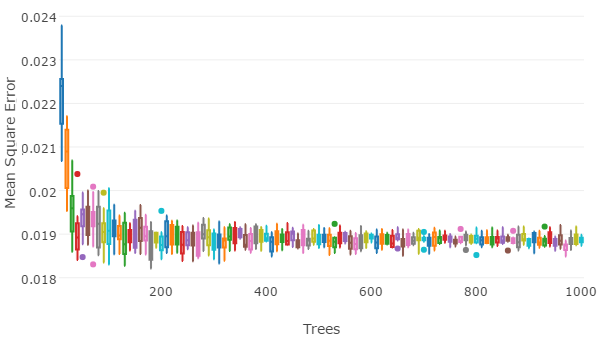
\includegraphics[height=1.2in]{RF_analysis/mse_trees.png} 
				\caption{Box plot : MSE with increasing number of trees}
			\end{subfigure}%
			~ 
			\begin{subfigure}[t]{0.5\textwidth}
				\label{figure:timing_trees}
				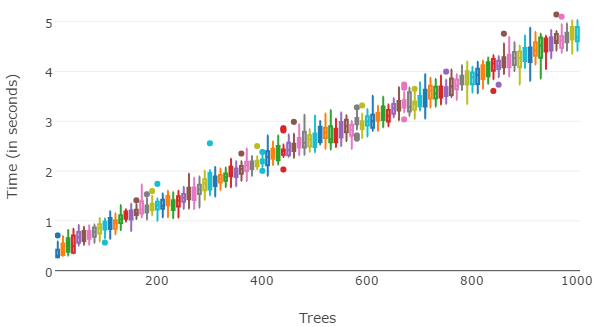
\includegraphics[height=1.2in]{RF_analysis/timing_trees.png} 
				\caption{Time with Trees increasing}
			\end{subfigure}
			\caption{Caption place holder}
		\end{figure*}
		
		
		\subsubsection{Out of Bag sampling}
		
		\subsubsection{Depth of the trees}
		
		\begin{figure}[H]
			\label{figure:mse_leaves}
			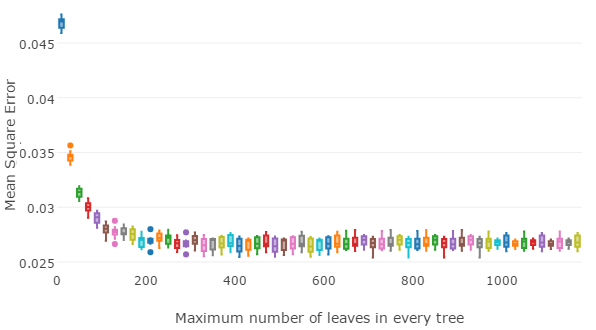
\includegraphics[scale=0.8]{RF_analysis/mse_leaves.png} 
			\caption{Box plot giving the mean square error given by Random forest with increasing number of features}
		\end{figure}
		
		\subsubsection{Variable Importance and features selection} 
		
		
		\paragraph{Tuning the max\_features hyperparameter}
		
		
		\begin{figure}[H]
			\label{figure:mse_feature}
			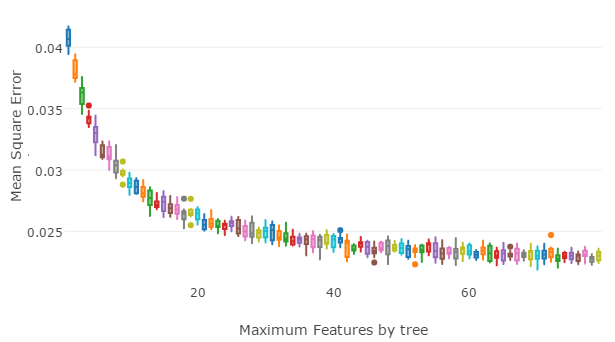
\includegraphics[scale=0.8]{RF_analysis/mse_features.png} 
			\caption{Box plot giving the mean square error of regression given by Random forest with increasing number of features}
		\end{figure}
		
		
		
		\begin{figure}[H]
			\label{figure:timing_features}
			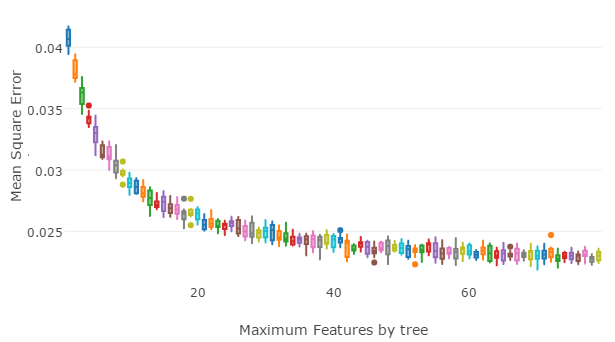
\includegraphics[scale=0.8]{RF_analysis/mse_features.png} 
			\caption{Box plot giving the mean square error with increasing number of trees}
		\end{figure}
		=
		
		\paragraph{Selecting the best features : Variable Importance}
		
		One can reduce the high dimensionality of a regression problem by selecting the 'best' features.
		
		Measuring this so called \textit{Variable Importance} makes it possible to rank the features by their importance. The difficult part here is the way to measure a feature's impact on the regression model. 
		Intuitively, the more an input $X_i$ is important, the worse the accuracy when removing it from the regression. 
		
		Thus when training a tree, it can be computed how much each feature decreases the impurity in a tree, called impurity score and known as \textit{Gini impurity} for classification and variance for regression.
		
		here method in \textit{Scikit-Learn} Random Forest Regressor class gives this information. 
		Drawing in the previous example a variable importance histogram gives
		
		\begin{figure}[H]
			\label{figure:vi}
			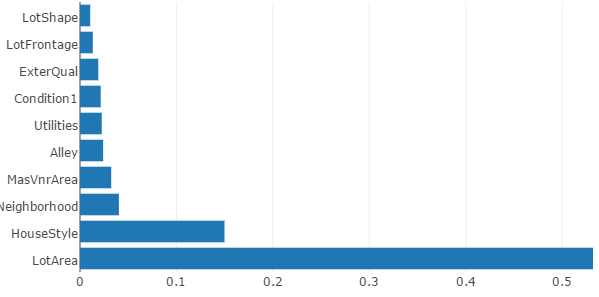
\includegraphics[scale=0.6]{RF_analysis/vi.png} 
			\caption{First ten most important variables given by Random Forest}
		\end{figure}
		
		Obviously the \textit{LotArea} represents the most important variable here.  
		
		
		
		Had it been that easy, we would then select the best features and rerun a Random Forest. 
		But, redundant information between features affects impurity measurements and thus its ranking. 
		This is not an issue for prediction and avoiding over fitting, but can lead to misinterpretation about a label importance. 
		\newline
		For instance
		
		\begin{Ex}
			let $X_0$, $X_1$, $X_2$,  $X_3$, $X_4$ and $X_5$ be six random variables having Gaussian distribution with mean 0 and variance 1.
			To add some correlation, we choose to add $X_0$ to every $X_i$,  $\forall i \in \{1,\cdots, 5\}$. 
			Let $Y$ be the sum of the correlated random variables $X_i$, $\forall i \in \{1,\cdots, 5\}$, i.e $Y = \sum_{i=1}^{5} X_i$. 
			It is clear here every input $X_i$ has the same impact on the output $Y$. 
			However, computing a Random Forest on $10.000$ samples of $(X, Y)$, $X$ being the concatenate of $X_i$, $i \in \{1,\cdots, 5\}$, gives the following Variable Importance bar plot
			\begin{figure}[H]
				\centering
				\label{figure:vi_ce}
				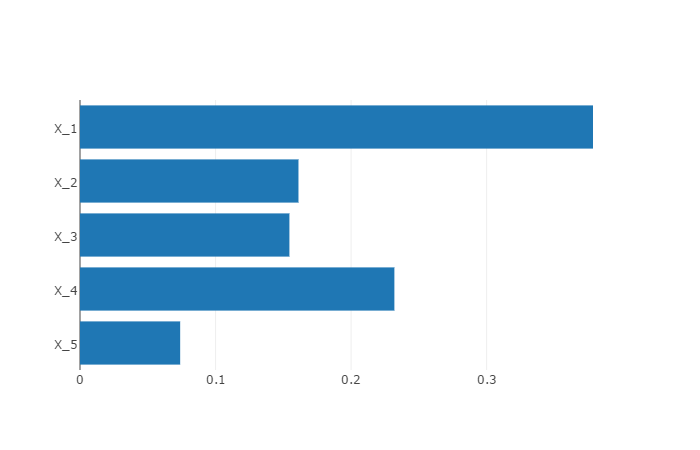
\includegraphics[scale=0.4]{RF_analysis/vi_contre_example.png} 
				\caption{Variable Importance with 5 correlated features $X_i$,$i \in \{1,\cdots, 5\}$ respectively taking importances 0.3785, 0.1612, 0.1545, 0.2319, 0.0739.}
			\end{figure}
			
			$X_1$ is five times 'more important' than $X_5$, which does not correspond to reality, as all inputs have the same impact on output $Y$. Random Forest seems to keep in 'mind' the information it gets, and if not needed, it does reduce its importance.  
			
		\end{Ex}
		
		Let's analyse this on the previous housing example :
		
		First, let's draw the correlation matrix between the inputs (we draw only a part here for better visualization): 
		
		\begin{figure}[!h]
			\label{figure:correlation_matrix}
			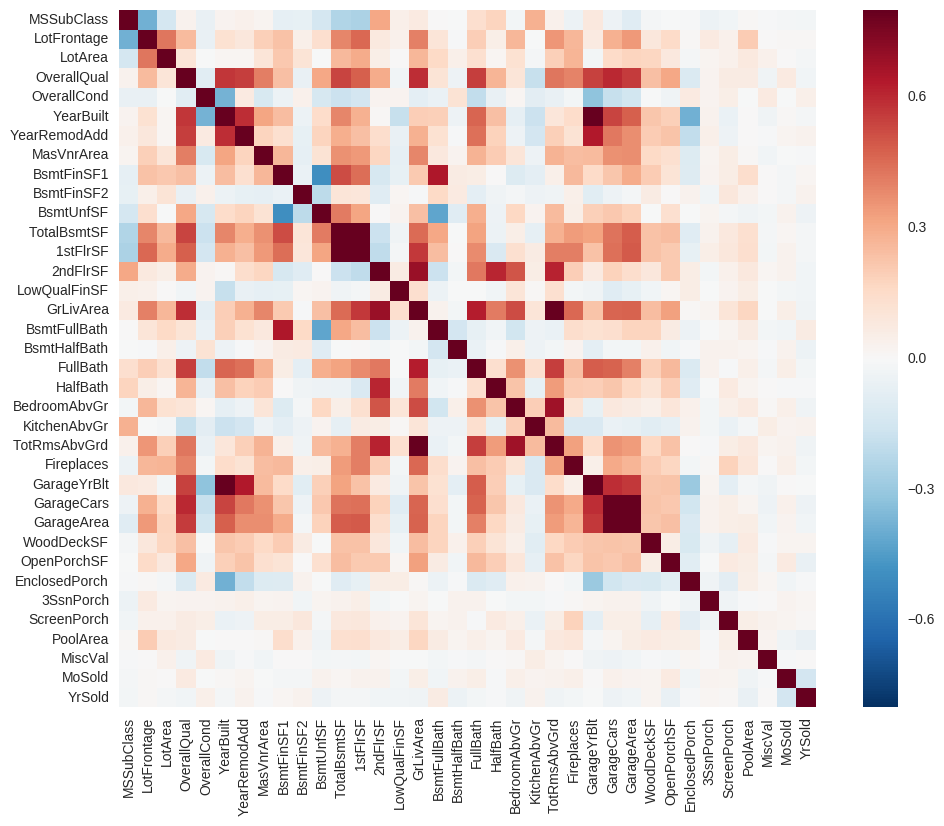
\includegraphics[scale=0.6]{RF_analysis/correlation_matrix.png} 
			\caption{Correlation matrix between the features of our housing market data}
		\end{figure}
		
		We can see \textit{LotFrontage}(Linear feet of street connected to property) and \textit{LotArea}("Lot size in square feet") are highly correlated (intuitively and by matrix correlation).
		However, growing a Random Forest gives the following Variable Importance ranking
		
		
		\section{Model Assessment and Selection}
		
		Inspired by Hastie, Tibshirani and Friedman \cite{Friedman:2008}, we present and describe variables used for regression model accuracy measurements.  
		These key methods enabled the comparisons made during financial applications in part 4. 
		
		\subsubsection{Bias and Variance}
		
		First tool of measurement is the precision of the model, called bias. Given a target variable $Y$, features $X = (X_1, \cdots, X_p$) and a regression model $\hat{f}$, estimated from a sample set $\mathcal{S}$, we denote $\mathcal{L}$ the loss function, measuring prediction errors between $Y$ and $\hat{f}(X)$, and defined by 
		
		\begin{displaymath}
		\mathcal{L}(Y, \hat{f}(X)) = ||Y - \hat{f}(X)||^2
		\end{displaymath}
		
		
	\end{appendices}
	
	\newpage
	\blankpage
	\bibliography{biblio}
	\bibliographystyle{plain}
	
\end{document}